\documentclass[10pt,aspectratio=169]{beamer} %class
\setbeamercovered{invisible}
\setbeamercovered{%
  again covered={\opaqueness<1->{15}}}
\usetheme[progressbar=frametitle]{metropolis} %theme
\usepackage{xcolor}
\usepackage{listings}

\lstset{language=C++,
                basicstyle=\ttfamily,
                keywordstyle=\color{blue}\ttfamily,
                stringstyle=\color{red}\ttfamily,
                commentstyle=\color{green}\ttfamily,
                morecomment=[l][\color{magenta}]{\#}
}


% Useful packages
\usepackage{appendixnumberbeamer}
\usepackage{booktabs}
\usepackage[scale=2]{ccicons}
\usepackage{calc}
\usepackage{pgfplots}
\usepgfplotslibrary{dateplot}
\usepackage{xspace}
\newcommand{\themename}{\textbf{\textsc{metropolis}}\xspace}

% define \hide command
\usepackage{xcolor}
\definecolor{hiddencolor}{HTML}{c4c4c4}
\newcommand{\hide}[1] {
	\textcolor{hiddencolor}{#1}
}

% Metadata
\title{Project Two}
\subtitle{Parallel computation of statistical values}
%\date{\today}
\date{}
\author{Blair Cox, Logan Small and Michael Kemp}
\institute{Group 12 - ParaStats}
%\titlegraphic{\hfill\includegraphics[height=1.5cm]{logo.pdf}}

% Begin document section
\begin{document}

% Title slide
\maketitle

% Table of contents slide
% \begin{frame}{Table of contents}
%   \setbeamertemplate{section in toc}[sections numbered]
%   \tableofcontents[hideallsubsections]
% \end{frame}

%%%%%%%%%%%%%%%%
% INTRODUCTION %
%%%%%%%%%%%%%%%%

\section{Introduction}
\begin{frame}[t]{Problem Context}
\vspace{3em}

\emph{``When working with data sets created from \alert{natural processes}, it is often important to get statistical values for these datasets. This assignment requires you to implement the calculation of statistical values over large data sets in parallel, for example the average, median, standard deviation etc."}

\vfill
\begin{itemize}
\item \alert{Natural processes} - A data stream of continuous values that are measuring events in nature.
\end{itemize}

\end{frame}

\begin{frame}[t]{Problem Context}
\vspace{3em}

\emph{``When working with data sets created from natural processes, it is often important to get \alert{statistical values} for these datasets. This assignment requires you to implement the calculation of statistical values over large data sets in parallel, for example the average, median, standard deviation etc."}

\vfill
\begin{itemize}
\item \alert{Statistical values} - Descriptive statistics that summarise a data set through representative scalar values.
\end{itemize}

\end{frame}

\begin{frame}[t]{Problem Context}
\vspace{3em}

\emph{``When working with data sets created from natural processes, it is often important to get statistical values for these datasets. This assignment requires you to implement the calculation of statistical values over \alert{large data sets} in parallel, for example the average, median, standard deviation etc."}

\vfill
\begin{itemize}
\item  \alert{Large data sets} - Large amounts of data that would be inefficient to process through normal means.
\end{itemize}

\end{frame}

\begin{frame}{Approach}


\begin{columns}[onlytextwidth]
\column{\dimexpr\linewidth-90mm-5mm}
\begin{itemize}
\item \alert{Parallelism}
\item \hide{OpenCL}
\item \hide{On-line processing}
\end{itemize}

\column{90mm}
\large
Analysing subsets of the data and then using reduction to combine the results.
\end{columns}

\end{frame}

\begin{frame}{Approach}


\begin{columns}[onlytextwidth]
\column{\dimexpr\linewidth-85mm-5mm}
\begin{itemize}
\item \hide{Parallelism}
\item \alert{OpenCL}
\item \hide{On-line processing}
\end{itemize}

\column{85mm}
\large
Low level programming language which generates portable code for heterogeneous devices.

\end{columns}

\end{frame}

\begin{frame}{Approach}


\begin{columns}[onlytextwidth]
\column{\dimexpr\linewidth-90mm-5mm}
\begin{itemize}
\item \hide{Parallelism}
\item \hide{OpenCL}
\item \alert{On-line processing}
\end{itemize}

\column{90mm}
\large
Dividing the input file into processable chunks and streamlining them onto the devices.
\end{columns}

\end{frame}


%%%%%%%%%%
% OPENCL %
%%%%%%%%%%

\section{OpenCL}

\begin{frame}{Motivation for OpenCL}
Why does OpenCL exist?
\begin{itemize}
\item A modern system can contain multiple CPUs and GPUs
\item Different vendors created different standards for utilizing their devices.
\item It is difficult to utilize this heterogeneous platform for parallel computing
\item OpenCL lets you create a single portable program that runs on all devices in parallel
\end{itemize}
  
\end{frame}

\begin{frame}{What is OpenCL}
What is OpenCL?
\begin{itemize}
\item Standardised language that doesn't tie implementation to specific devices. 
\item It is a programming framework for parallel computing.
\item Runs instructions on acceleration units irregardless of hardware specifications.
\end{itemize}
  
\end{frame}

%%Core Concepts
\begin{frame}{Platform Model}

\begin{columns}[onlytextwidth]
\column{\dimexpr\linewidth-80mm-5mm}
\begin{itemize}
\item Made up of a host, and multiple OpenCL devices %Use an example to explain (slide27)
\item These devices are comprised of multiple compute units, and these compute units consist of processing elements.
\end{itemize}

\column{80mm}
\begin{figure}
    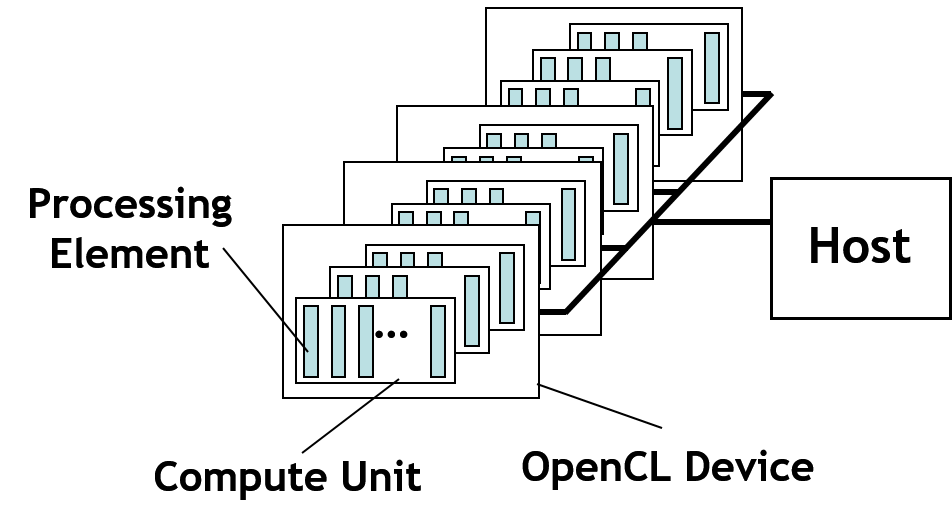
\includegraphics[width=\textwidth]{PlatformModel.png}
    \caption{Platform Model \emph{\textcopyright \scriptsize\raise0.35ex\hbox{Khronos Group, 2013}}}
\end{figure}
\end{columns}
  
\end{frame}

\begin{frame}[fragile,t]{Data parallelism}
\vspace{1em}
Translate loops to functions (kernels) which operate on every data point in the problem domain
\vspace{1em}
\begin{columns}[t]
\begin{column}{0.5\textwidth}
\alert{C Loop}
\begin{lstlisting}
  void add(
    const int n,
    const float* a,
    const float* b,
    float* c)
  {
    for (int i = 0; i < n; i++)
        c[i] = a[i] + b[i];
  }
\end{lstlisting}
\end{column}%
\hspace{-10pt}
\vrule{}%
\hspace{15pt}
\begin{column}{0.5\textwidth}
\phantom{
OpenCL Kernel
  \_\_kernel void vadd(                             
     \_\_global float* a,                      
     \_\_global float* b,                      
     \_\_global float* c,                      
     const int count)               
  \{                                          
     int i = get\_global\_id(0);
     c[i] = a[i] + b[i];
  \}   
  }
\end{column}
\end{columns}
\end{frame}


\begin{frame}[fragile,t]{Data parallelism}
\vspace{1em}
Translate loops to functions (kernels) which operate on every data point in the problem domain
\vspace{1em}
\begin{columns}[t]
\begin{column}{0.5\textwidth}
\alert{C Loop}
\begin{lstlisting}
  void add(
    const int n,
    const float* a,
    const float* b,
    float* c)
  {
    for (int i = 0; i < n; i++)
        c[i] = a[i] + b[i];
  }
\end{lstlisting}
\end{column}%
\hspace{-10pt}
\vrule{}%
\hspace{15pt}
\begin{column}{0.5\textwidth}
\alert{OpenCL Kernel}
\begin{lstlisting}
  __kernel void add(                             
     __global float* a,                      
     __global float* b,                      
     __global float* c)               
  {                                          
     int i = get_global_id(0);
     c[i] = a[i] + b[i];
  }   
  
  \end{lstlisting}
\end{column}
\end{columns}
\end{frame}

\begin{frame}{N-Dimensional Work Domain}
\begin{columns}[c]
\begin{column}{0.5\textwidth}
\begin{itemize}
\item When we structure the problem domain, we specify up to 3 dimensions and their sizes
\item Each point in the specified domain is mapped to a work-item
\item Work-items are grouped into work-groups which share local memory
\end{itemize}
\end{column}%
\begin{column}{0.5\textwidth}
\begin{figure}
    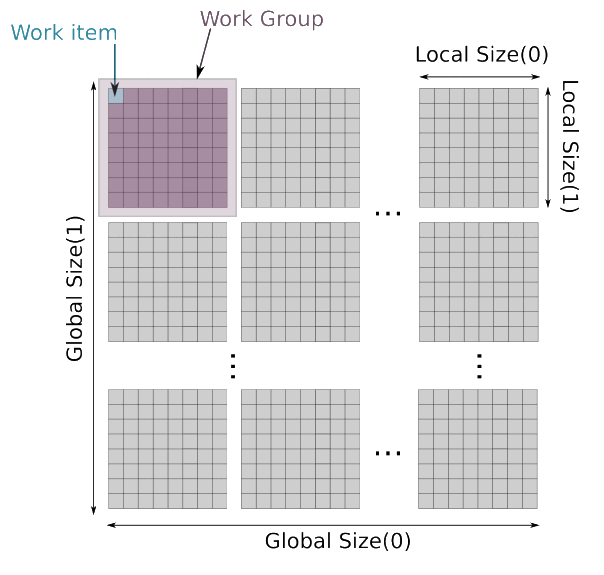
\includegraphics[width=\textwidth]{WorkGI.png}
    \caption{Work Item/Group Layout \textsuperscript{\cite{Hong2016}}}
\end{figure}
\end{column}
\end{columns}
  
\end{frame}

\begin{frame}{Memory Model}
\begin{columns}[c]
\begin{column}{0.48\textwidth}
\begin{enumerate}
\item[] \makebox[6.8em][l]{Work-item} \makebox[2em][r]{$\longrightarrow$}  \makebox[7.5em][r]{Private Memory}
\item[] \makebox[6.8em][l]{Work-group} \makebox[2em][r]{$\longrightarrow$}  \makebox[7.5em][r]{Local Memory}
\item[] \makebox[6.8em][l]{Compute Device} \makebox[2em][r]{$\longrightarrow$}  \makebox[7.5em][r]{Global Memory}
\item[] \makebox[6.8em][l]{Host Device} \makebox[2em][r]{$\longrightarrow$}  \makebox[7.5em][r]{Host Memory}
\end{enumerate}
\end{column}
\begin{column}{0.52\textwidth}
\begin{figure}
    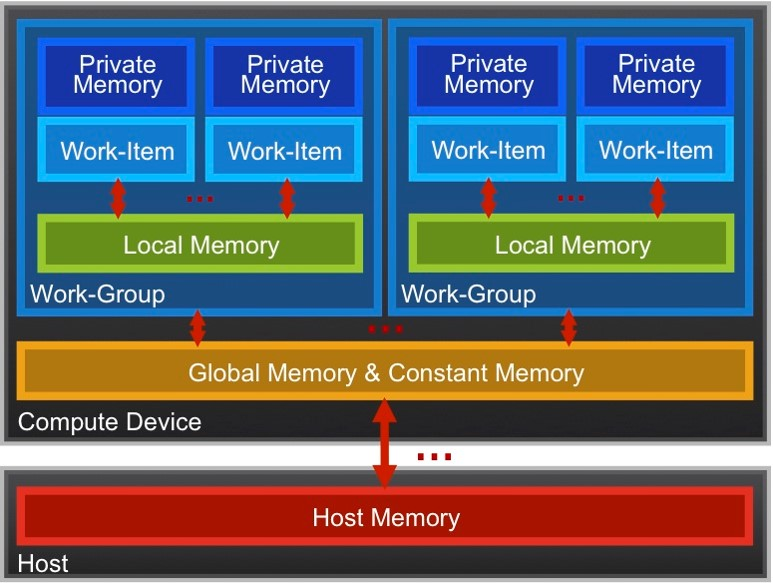
\includegraphics[width=\textwidth]{OpenCLMemModel.jpg}
    \caption{OpenCL Memory Model \emph{\textcopyright \scriptsize\raise0.35ex\hbox{Khronos Group, 2013}}}
\end{figure}
\end{column}
\end{columns}
\end{frame}



\begin{frame}{GPU vs CPU}

\begin{columns}[c]
\begin{column}{0.4\textwidth}
\begin{itemize}[<+- | alert@+>]
\item Matrix multiplication performance
%\item Work Item vs Work Group
\item Structure of Arrays vs Array of Structures
\end{itemize}
\end{column}%
\begin{column}{0.6\textwidth}
\begin{figure}
    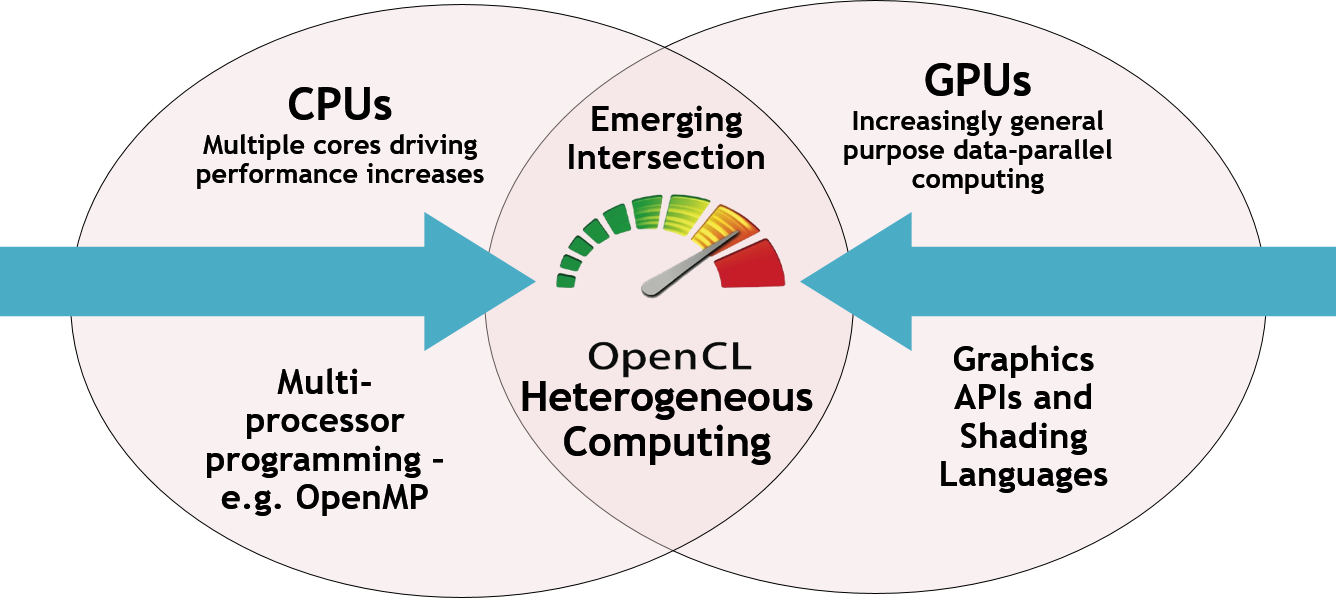
\includegraphics[width=\textwidth]{gpucpu.png}
    \caption{GPU vs CPU \emph{\textcopyright \scriptsize\raise0.35ex\hbox{Khronos Group, 2013}}}
\end{figure}
\end{column}
\end{columns}
\end{frame}
	
\begin{frame}[fragile,t]{Host \& Device Code}
\vspace{1.5em}
\begin{columns}[t]
\begin{column}{0.5\textwidth}
\alert{Host code using C++ Bindings}
\begin{lstlisting}
  cl::make_kernel<cl::Buffer,
  cl::Buffer, cl::Buffer,
  <int> vadd(program, "vadd");

  d_a = cl::Buffer(context,
  h_a.begin(), h_a.end(), true);

  vadd(
       cl::EnqueueArgs(queue,
          cl::NDRange(count)), 
       d_a,
       count);
\end{lstlisting}
\end{column}%
\hspace{-10pt}
\vrule{}%
\hspace{15pt}
\begin{column}{0.5\textwidth}
\alert{Device code (Kernel)}
\begin{lstlisting}
  __kernel void vadd(                             
     __global float* a,                      
     __global float* b,                      
     __global float* c)               
  {                                          
     int i = get_global_id(0); 
     c[i] = a[i] + b[i];
  }   
\end{lstlisting}
\end{column}
\end{columns}
\end{frame}


%%%%%%%%%
% STATS %
%%%%%%%%%

\section{Statistical Algorithms}

\begin{frame}{Summary Statistics}
\begin{columns}[c]
\begin{column}{0.35\textwidth}
\begin{itemize}
\item \alert{Measures of Location }
\item \hide{Measures of Spread}
\item \hide{Measures of Shape}
\item \hide{Multivariate Statistics}
\end{itemize}
\end{column}

\begin{column}{0.65\textwidth}
\begin{figure}
    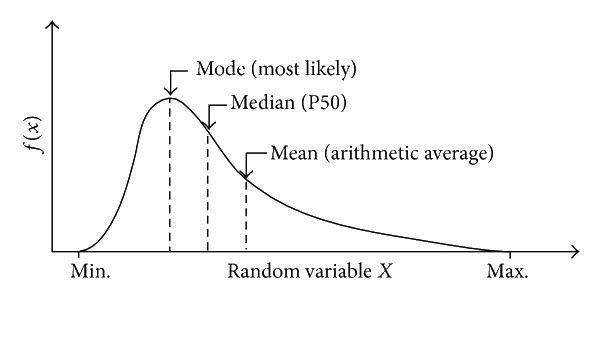
\includegraphics[width=\textwidth]{measure_location.png}
    \caption{Central Tendency}
\end{figure}
\end{column}
\end{columns}
\end{frame}

\begin{frame}{Summary Statistics}
\begin{columns}[c]
\begin{column}{0.35\textwidth}
\begin{itemize}
\item \hide{Measures of Location}
\item \alert{Measures of Spread}
\item \hide{Measures of Shape}
\item \hide{Multivariate Statistics}
\end{itemize}
\end{column}

\begin{column}{0.65\textwidth}
\begin{figure}
    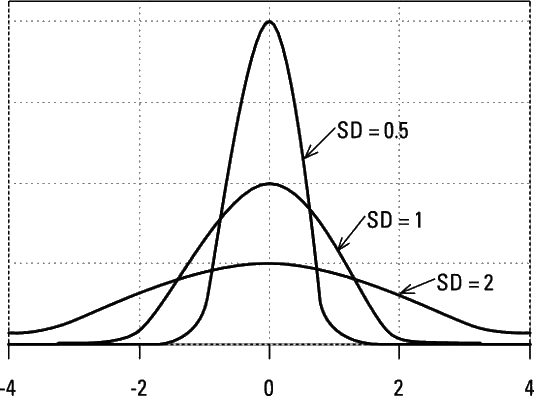
\includegraphics[width=0.8\textwidth]{measure_spread.png}
    \caption{Standard Deviation}
\end{figure}
\end{column}
\end{columns}
\end{frame}

\begin{frame}{Summary Statistics}
\begin{columns}[c]
\begin{column}{0.35\textwidth}
\begin{itemize}
\item \hide{Measures of Location}
\item \hide{Measures of Spread}
\item \alert{Measures of Shape}
\item \hide{Multivariate Statistics}
\end{itemize}
\end{column}

\begin{column}{0.65\textwidth}
\begin{figure}
    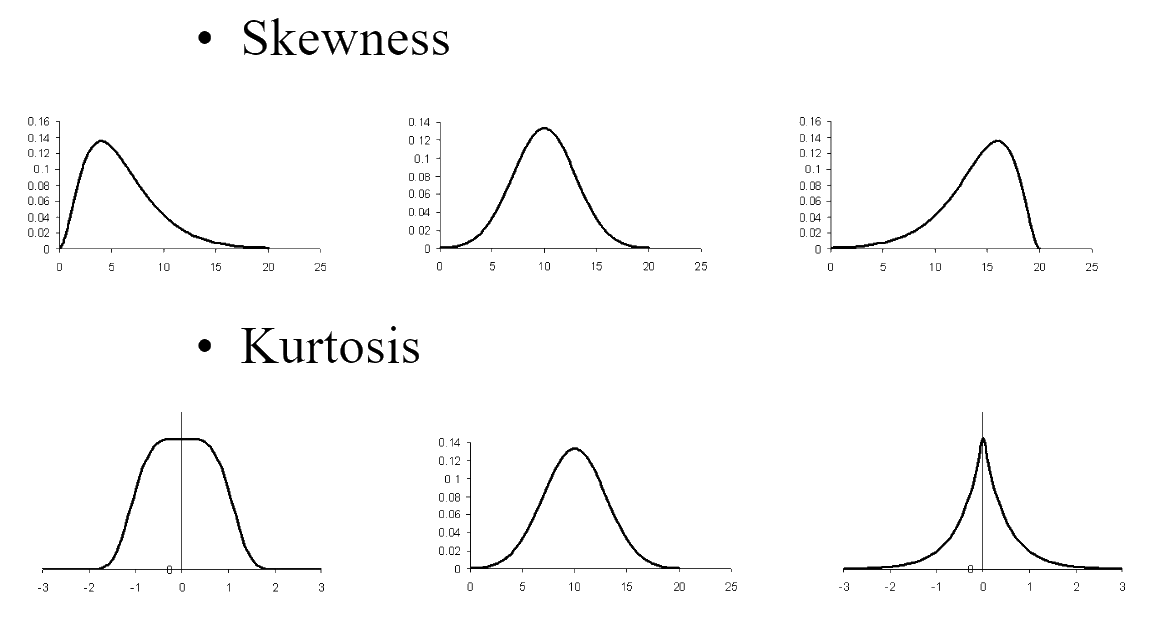
\includegraphics[width=0.8\textwidth]{measure_shape.png}
    \caption{Skewness and Kurtosis}
\end{figure}
\end{column}
\end{columns}
\end{frame}

\begin{frame}{Summary Statistics}
\begin{columns}[c]
\begin{column}{0.35\textwidth}
\begin{itemize}
\item \hide{Measures of Location}
\item \hide{Measures of Spread}
\item \hide{Measures of Shape}
\item \alert{Multivariate Statistics}
\end{itemize}
\end{column}

\begin{column}{0.65\textwidth}
Assumption: We are dealing with only one variable
\end{column}
\end{columns}
\end{frame}

\begin{frame}{Fundamental Values}

The minimal statistical model from which all relevant summary statistics can be derived:
\begin{columns}[c]
\begin{column}{0.4\textwidth}
\begin{itemize}
\item Sample size
\item Moment 1
\item Moment 2
\item Moment 3
\item Moment 4
\item Rank
\item Min/Max
\item Histogram
\end{itemize}
\end{column}
\begin{column}{0.6\textwidth}
\begin{figure}
    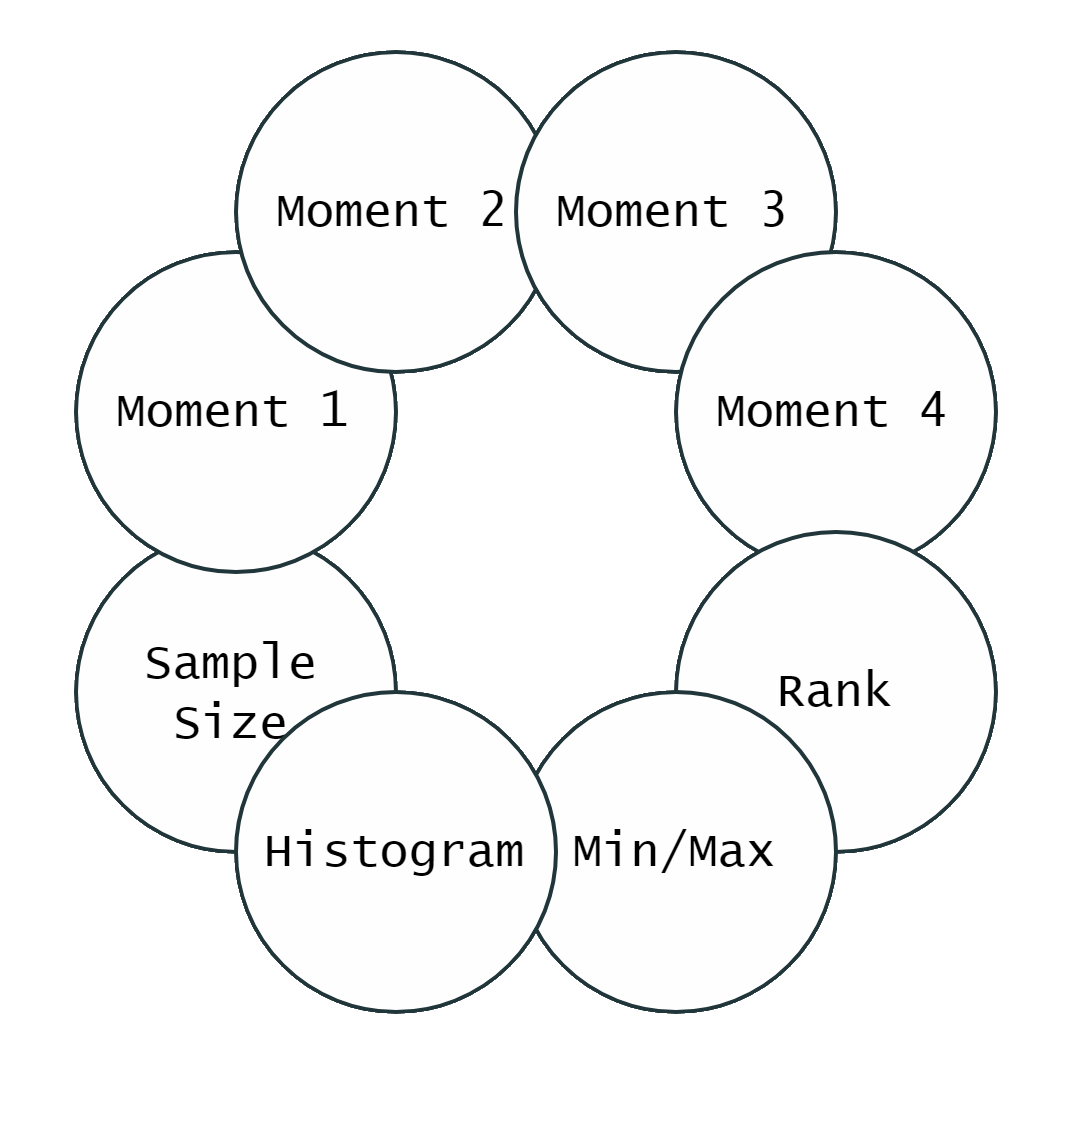
\includegraphics[width=0.68\textwidth]{fundamental.png}
    \caption{Minimal Statistical Model}
\end{figure}
\end{column}
\end{columns}
\end{frame}

\begin{frame}{Derived Values}
From the fundamental values, we can derive all widely used summary statistics
\begin{figure}
    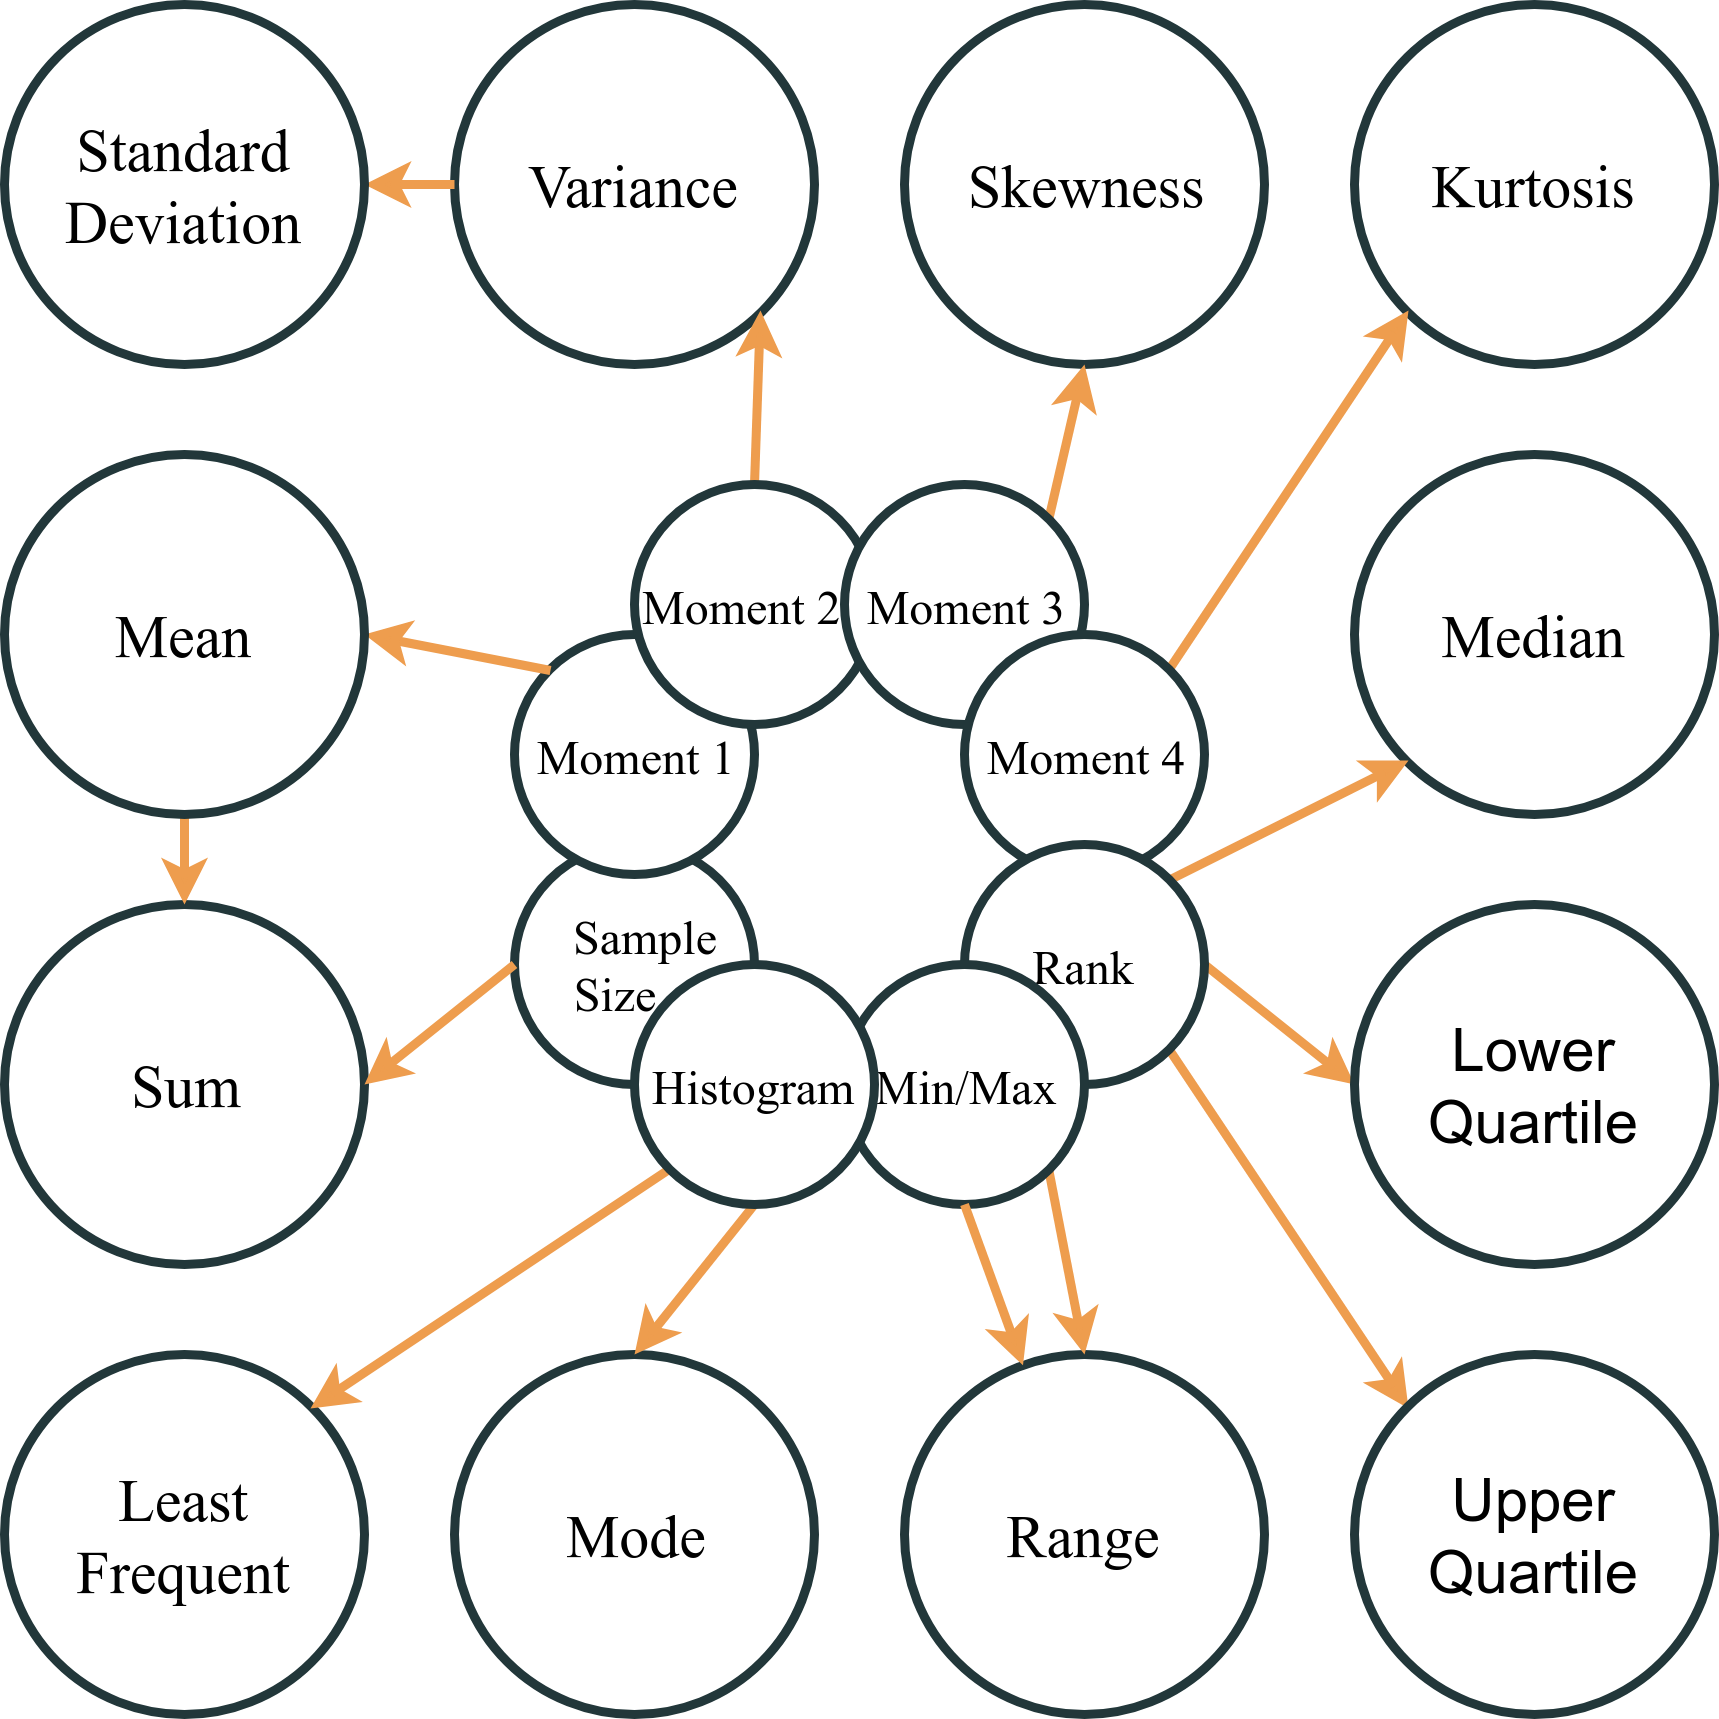
\includegraphics[height=0.74\textheight]{Extended.png}
    \caption{Extended Statistical Model}
\end{figure}
\end{frame}

\begin{frame}{On-line Algorithms}
\begin{columns}[c]
\begin{column}{0.5\textwidth}
\begin{itemize}
\item Sample Size - Count on host
\item Moments - Equations on Right
\item Rank (Median, etc) - Selection Algorithm
\item Min/Max - Per-element update
\item Histogram - Frequency Analysis
\end{itemize}
\end{column}
\begin{column}{0.5\textwidth}
\begin{figure}
    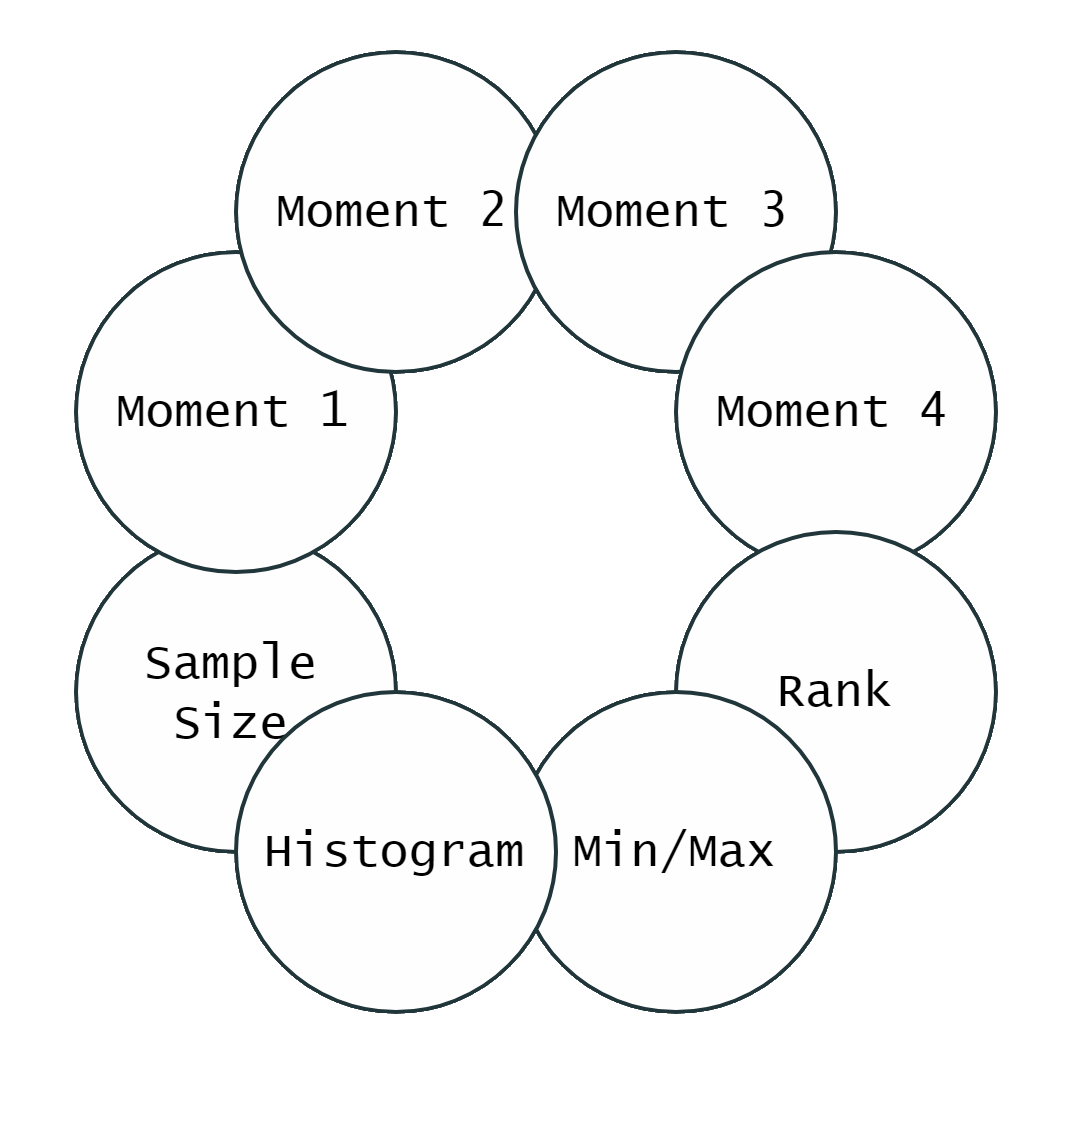
\includegraphics[width=0.68\textwidth]{fundamental.png}
    \caption{Minimal Statistical Model}
\end{figure}
\end{column}
\end{columns}
\end{frame}

\begin{frame}{On-line Algorithms}
\begin{columns}[c]
\begin{column}{0.5\textwidth}
\begin{itemize}
\item \alert{Sample Size - Count on host}
\item \hide{Moments - Equations on Right}
\item \hide{Rank (Median, etc) - Selection Algorithm}
\item \hide{Min/Max - Per-element update}
\item \hide{Histogram - Frequency Analysis}
\end{itemize}
\end{column}
\begin{column}{0.5\textwidth}
As we know the size of the arrays that we are sending to the devices, it is useless to count the data points using OpenCL
\end{column}
\end{columns}
\end{frame}

\begin{frame}{On-line Algorithms}
\begin{columns}[c]
\begin{column}{0.5\textwidth}
\begin{itemize}
\item \hide{Sample Size - Count on host}
\item \alert{Moments - Equations on Right}
\item \hide{Rank (Median, etc) - Selection Algorithm}
\item \hide{Min/Max - Per-element update}
\item \hide{Histogram - Frequency Analysis}
\end{itemize}
\end{column}
\begin{column}{0.5\textwidth}
\begin{figure}
	{
	\setlength{\fboxsep}{1pt}%
	\setlength{\fboxrule}{1pt}%
	\fbox{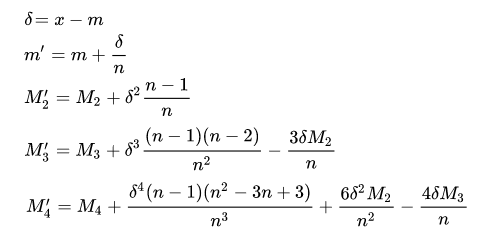
\includegraphics[width=\textwidth]{equations.png}}%
	}%
    \caption{Moment Equations \cite{Pebay2008}}
\end{figure}
\end{column}
\end{columns}
\end{frame}

\begin{frame}{On-line Algorithms}
\begin{columns}[c]
\begin{column}{0.5\textwidth}
\begin{itemize}
\item \hide{Sample Size - Count on host}
\item \hide{Moments - Equations on Right}
\item \alert{Rank (Median, etc) - Selection Algorithm}
\item \hide{Min/Max - Per-element update}
\item \hide{Histogram - Frequency Analysis}
\end{itemize}
\end{column}
\begin{column}{0.5\textwidth}
$k^{th}$ smallest element in a stream - partial sorting
\end{column}
\end{columns}
\end{frame}

\begin{frame}{On-line Algorithms}
\begin{columns}[c]
\begin{column}{0.5\textwidth}
\begin{itemize}
\item \hide{Sample Size - Count on host}
\item \hide{Moments - Equations on Right}
\item \hide{Rank (Median, etc) - Selection Algorithm}
\item \alert{Min/Max - Per-element update}
\item \hide{Histogram - Frequency Analysis}
\end{itemize}
\end{column}
\begin{column}{0.5\textwidth}
Compare each data point to a `running min/max' and update
\end{column}
\end{columns}
\end{frame}

\begin{frame}{On-line Algorithms}
\begin{columns}[c]
\begin{column}{0.5\textwidth}
\begin{itemize}
\item \hide{Sample Size - Count on host}
\item \hide{Moments - Equations on Right}
\item \hide{Rank (Median, etc) - Selection Algorithm}
\item \hide{Min/Max - Per-element update}
\item \alert{Histogram - Frequency Analysis}
\end{itemize}
\end{column}
\begin{column}{0.5\textwidth}
\begin{figure}
    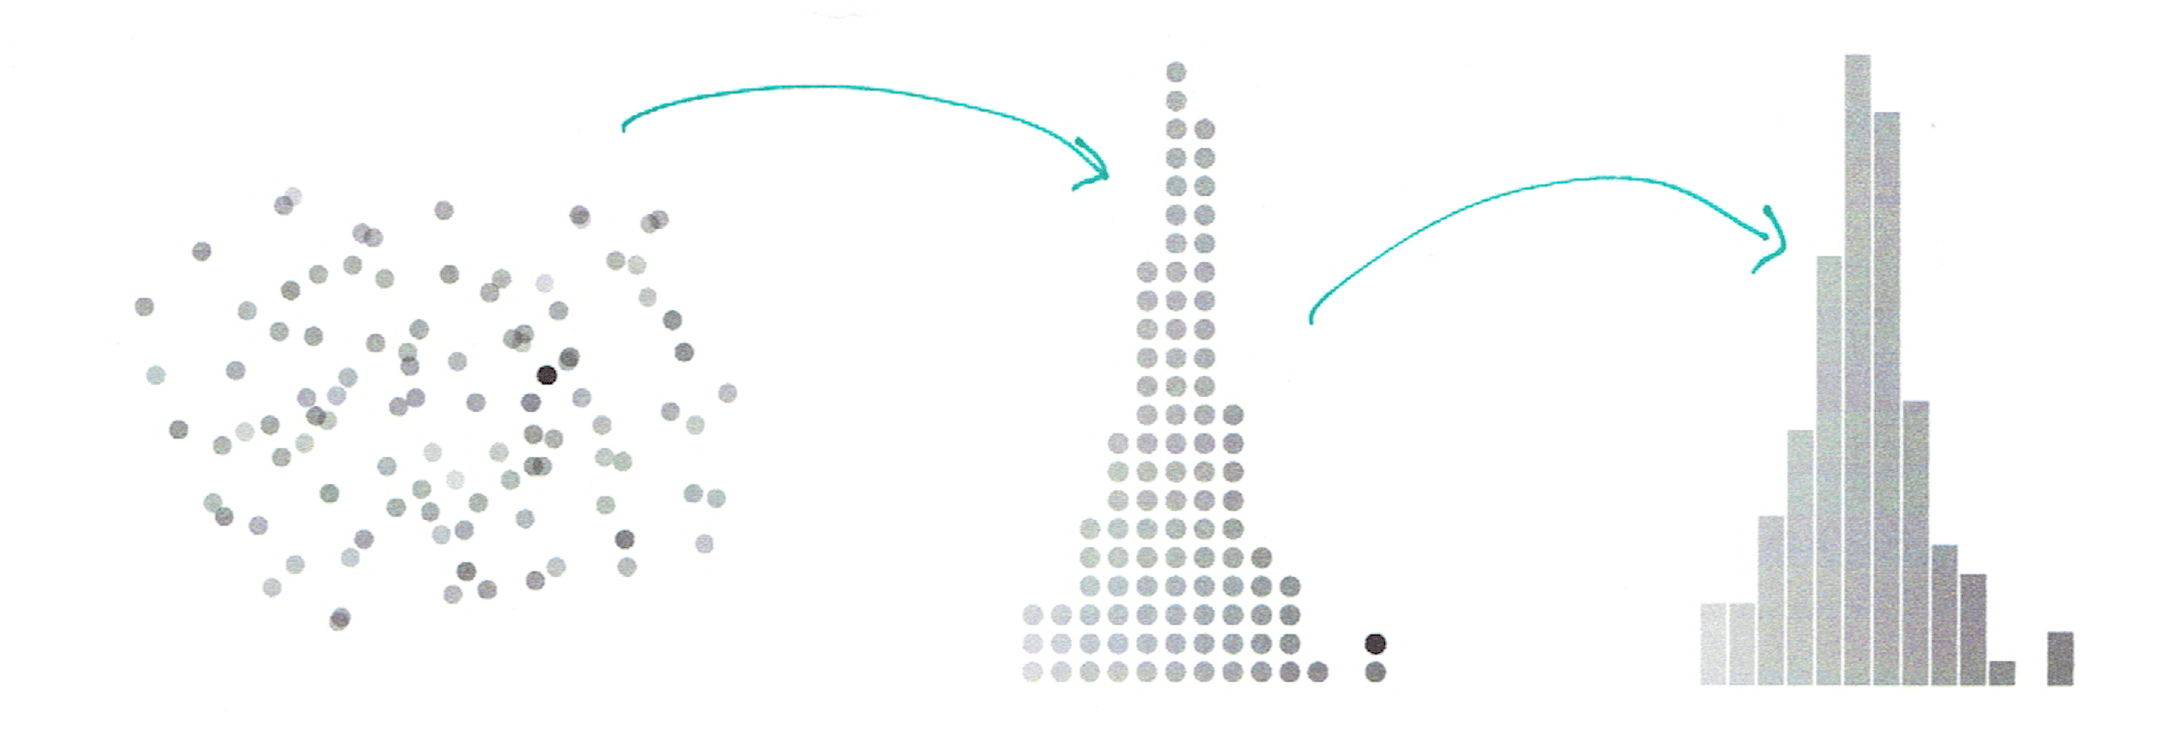
\includegraphics[width=\textwidth]{histogram.png}
    \caption{Histogram}
\end{figure}
\end{column}
\end{columns}
\end{frame}


%%%%%%%%%%%%%%%%%%
% IMPLEMENTATION %
%%%%%%%%%%%%%%%%%%

\section{Our Implementation (So Far)}

\begin{frame}{Sequential}
We can:
\begin{itemize}
\item Recalculate the base statistical values after every data-point
\item Could possibly move to recalculating in chunks (possibly target cache size)
\end{itemize}
Three types of statistics to calculate:
\begin{itemize}
\item Minimum, maximum, and sample size are trivial
\item Histogram (mode, etc.) and Rank (quartiles, median) use a HashMap
\item Moments (mean, etc.) recalculation use weighted average:
\end{itemize}
$$\frac{numValuesIn(a)\times a+numValuesIn(b)\times b}{numValuesIn(a) + numValuesIn(b)}$$
\end{frame}

\begin{frame}{Sequential: Results}
\centering{Ran 3 times on an i7-7500U with 8GB RAM and a MX300 SSD}
\begin{figure}
{
\setlength{\fboxsep}{1pt}%
\setlength{\fboxrule}{1pt}%
\fbox{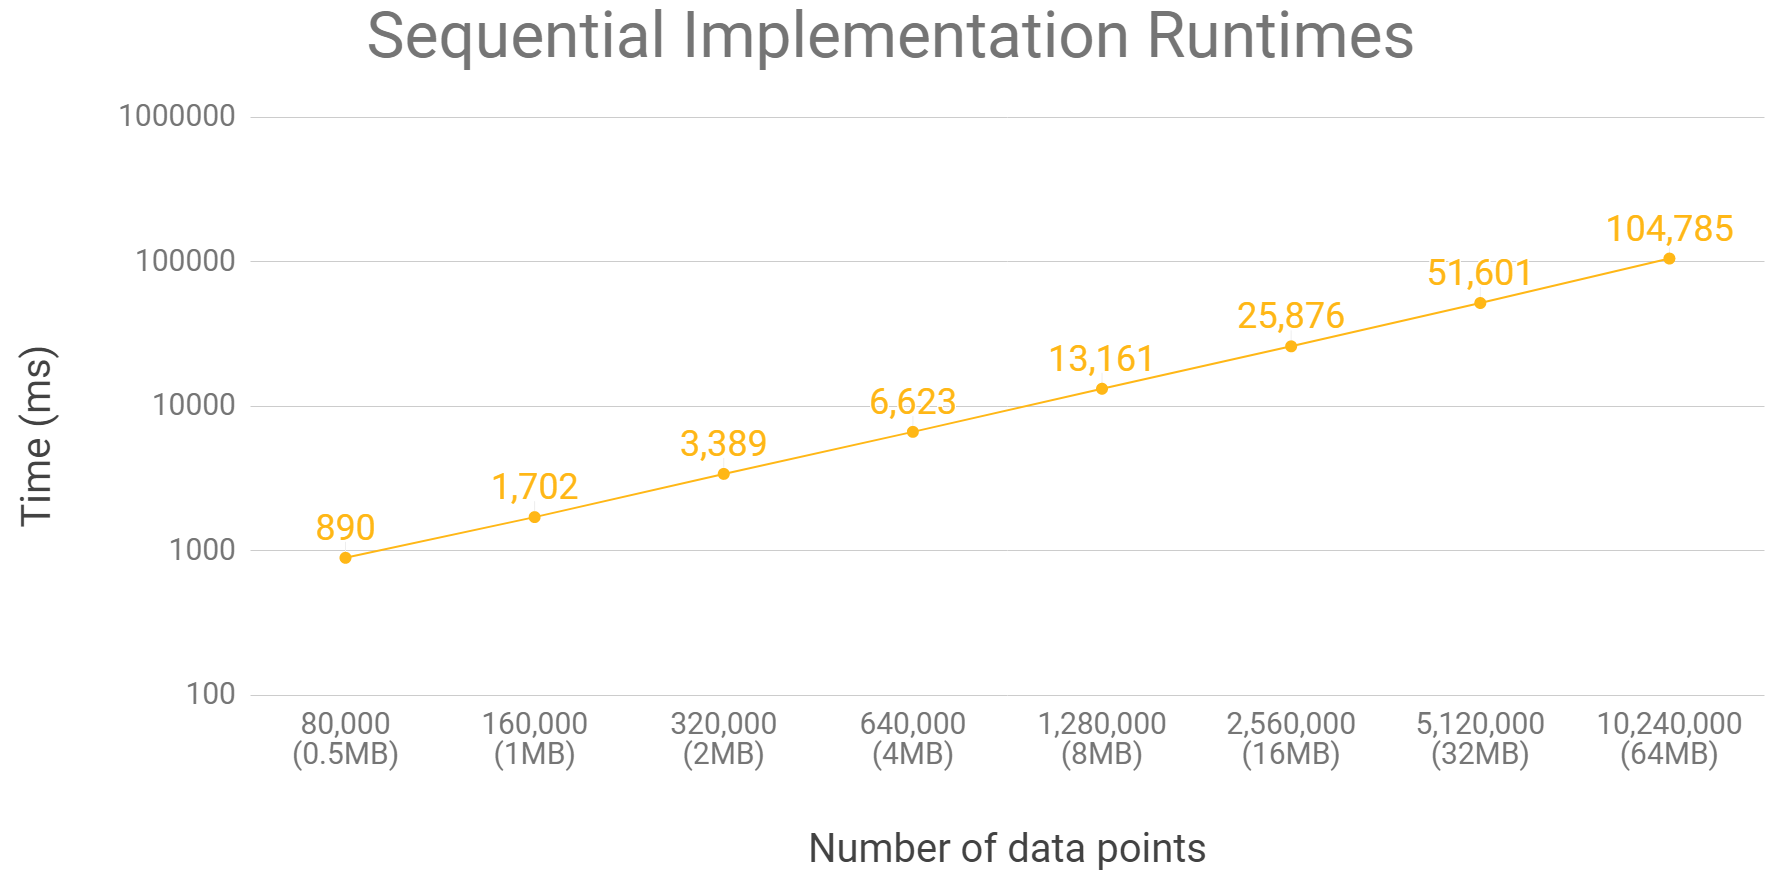
\includegraphics[width=0.8\textwidth]{Sequential_runtimes}}%
}%
\caption{Sequential Runtimes}
\end{figure}
\end{frame}

\begin{frame}{Sequential: Big Data}
To really test this we tried a much bigger data set
\begin{itemize}
	\item File-size: 4.2GiB
    \item Runtime: 37:32 (m:s)
    \item Data-points: 655,360,000
    \item Only run once (no averaging)
\end{itemize}
\end{frame}

\begin{frame}{Sequential: What we learned}
\begin{itemize}[<+- | alert@+>]
\item Linear runtime (each data-point is processed once) as expected
\item Can process hundreds of millions of data points
\item Reasonable time-frame but still slow
\item The L3 cache being loaded can be seen
\end{itemize}
\end{frame}

\begin{frame}{Parallel Implementation}
Calculation via reduction:
\begin{itemize}
\item Each work item is calculating on small number of points
\item Each work group reduces results of the work items
\item The final result is a reduction of the work groups
\end{itemize}
So far we've found GPUs can really improve performance
\end{frame}

\begin{frame}{Parallel \& Problems}
Here are the problems we found during implementation:
\begin{itemize}[<+- | alert@+>]
\item Reduction is hard in OpenCL (truly)
\item Memory needs to be explicitly shared
\item Synchronising work groups
\item Choosing work group and work item size
\item Can't optimise too hard
\end{itemize} 
\end{frame}

%%%%%%%%%%%%%%%
% FUTURE WORK %
%%%%%%%%%%%%%%%

\section{Future Work}



\begin{frame}{Optimisation}

\begin{columns}[onlytextwidth]
\column{\dimexpr\linewidth-85mm-5mm}
\begin{itemize}
\item \alert{Efficient Memory Access}
\item \hide{Local Memory}
\item \hide{Work Item Setup}
\item \hide{Occupancy}
\end{itemize}

\column{85mm}
\large
\begin{itemize}
\item Ideally we want all work items to access their data points at the same time, improving concurrency
\item Structure of arrays vs array of structures
\end{itemize}

\end{columns}
  
\end{frame}

\begin{frame}{Optimisation}

\begin{columns}[onlytextwidth]
\column{\dimexpr\linewidth-85mm-5mm}
\begin{itemize}
\item \hide{Efficient Memory Access}
\item \alert{Local Memory}
\item \hide{Work Item Setup}
\item \hide{Occupancy}
\end{itemize}

\column{85mm}
\large
The contradiction:
\begin{itemize}
\item Supposed to hold data reused by ALL work items to minimise memory movements $\Rightarrow$ performance
\item \alert{But} CPUs don't have special hardware and modern GPU caches can give the same effect
\end{itemize}

\end{columns}
  
\end{frame}

\begin{frame}{Optimisation}

\begin{columns}[onlytextwidth]
\column{\dimexpr\linewidth-85mm-5mm}
\begin{itemize}
\item \hide{Efficient Memory Access}
\item \hide{Local Memory}
\item \alert{Work Item Setup}
\item \hide{Occupancy}
\end{itemize}

\column{85mm}
\large
The optimal amount of work items per work group changes based on:
\begin{itemize}
\item the data set and
\item device architecture | GPU vs CPU (again)
\end{itemize}

\end{columns}
  
\end{frame}

\begin{frame}{Optimisation}

\begin{columns}[onlytextwidth]
\column{\dimexpr\linewidth-85mm-5mm}
\begin{itemize}
\item \hide{Efficient Memory Access}
\item \hide{Local Memory}
\item \hide{Work Item Setup}
\item \alert{Occupancy}
\end{itemize}

\column{85mm}
\large
Need every processing element on an OpenCL device to be active, a typical ``good'' measurement of occupancy is over 0.5
\end{columns}
  
\end{frame}

\begin{frame}{Testing}
//\alert{TODO: Test and compare the implementations }
\end{frame}

%%%%%%%%%%%%%%
% CONCLUSION %
%%%%%%%%%%%%%%

\section{Conclusion}

\begin{frame}{Summary}

\begin{itemize}
\item OpenCL
\item Summary Statistics
\begin{itemize}
\item Algorithms
\end{itemize}
\item Implementation
\begin{itemize}
\item Problems
\item Future Optimisation
\end{itemize}
\end{itemize}


\end{frame}

\begin{frame}[fragile]{Kahoot!\texttrademark}

\alert{Kahoot!\texttrademark  Quiz:}\\

\small
\url{https://play.kahoot.it/#/?quizId=11f98885-2501-4364-bc3c-247834e9f73d}
\normalsize

\end{frame}

%%%%%%%%%%%%%%%%%%%
% QUESTIONS SLIDE %
%%%%%%%%%%%%%%%%%%%
\begin{frame}[standout]
  Questions?
\end{frame}

%%%%%%%%%%%%%%%%%%%
% APPENDIX SLIDES %
%%%%%%%%%%%%%%%%%%%
\appendix

\section{Backup slides}


\begin{frame}[fragile]{Structure of Arrays vs Array of Structures}
\begin{lstlisting}
struct { float x, y, z, a; } Point; 
\end{lstlisting}
\begin{itemize}
\item SoA: GPU, Adjacent work items prefer adjacent memory because of Memory Cohesion
\item AoS: CPU, Individual work items prefer adjacent memory because of Cache Hierarchies 
\end{itemize}
\begin{figure}
    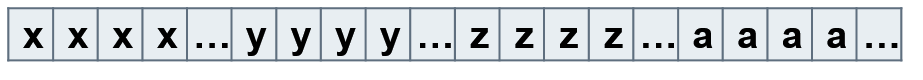
\includegraphics[width=0.8\textwidth]{soa.png}
    \caption{Structure of Arrays \emph{\textcopyright \scriptsize\raise0.35ex\hbox{Khronos Group, 2013}}}
\end{figure}
\begin{figure}
    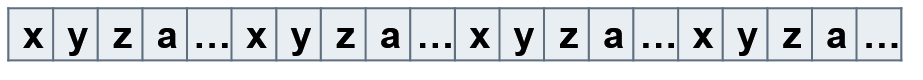
\includegraphics[width=0.8\textwidth]{Aos.png}
    \caption{Array of Structures \emph{\textcopyright \scriptsize\raise0.35ex\hbox{Khronos Group, 2013}}}
\end{figure}
\end{frame}

\begin{frame}{GPU vs CPU matrix multiplication}
\begin{figure}
    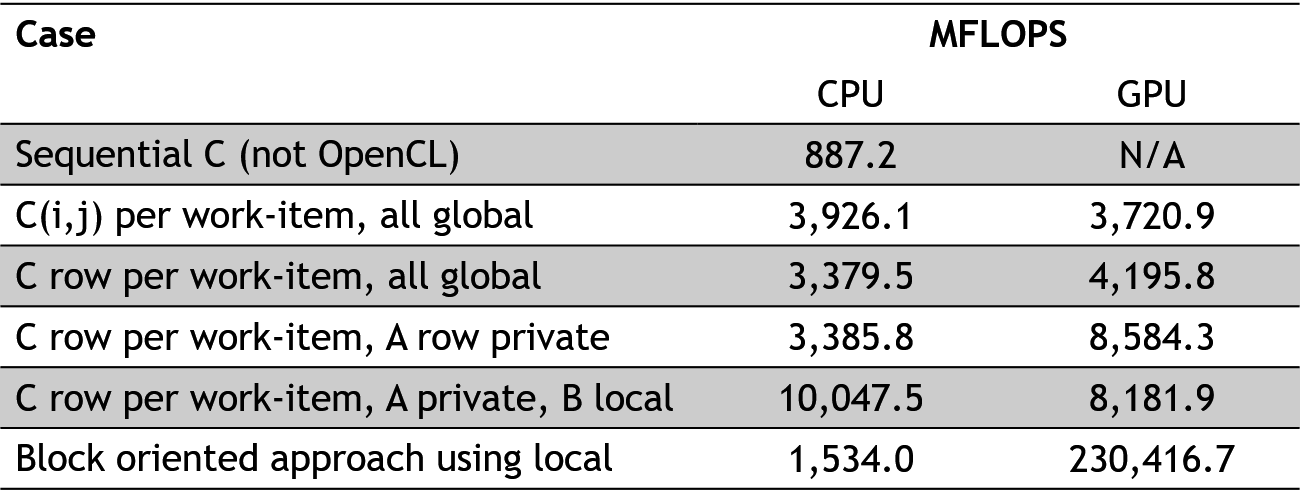
\includegraphics[width=0.8\textwidth]{MFlops.png}
    \caption{Different Multiplication Techniques \emph{\textcopyright \scriptsize\raise0.35ex\hbox{Khronos Group, 2013}}}
\end{figure}
\end{frame}

\begin{frame}{Main Concept Overview}
\begin{columns}[c]
\begin{column}{0.35\textwidth}
\begin{itemize}
\item N-D Range
\item Memory Model
\item Kernel and Host
\end{itemize}
\end{column}%
\begin{column}{0.65\textwidth}
\begin{figure}
    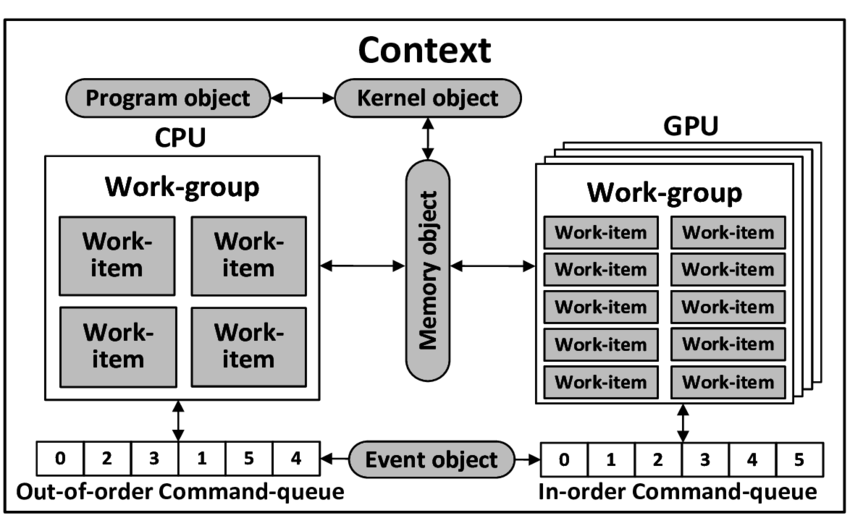
\includegraphics[width=\textwidth]{OpenCLOverall.png}
    \caption{OpenCL Execution Model \textsuperscript{ \cite{Stone2010}}}
\end{figure}
\end{column}
\end{columns}
\end{frame}

\begin{frame}{Terminology}

\begin{itemize}
\item Host - Program managing the compute devices
\item Kernel - Instructions for the compute devices
\item Work Item - An element of the problem
\item Work Group - Consists of work items
\item N-D Range - Organisation of kernel into N-Dimensional arrays of work groups
\end{itemize}
\end{frame}

\begin{frame}[allowframebreaks]{References}

  \bibliography{751presentation}
  \bibliographystyle{apalike}

\end{frame}

% End document section
\end{document}
